\documentclass[12pt]{article}
\usepackage[english]{babel}
\usepackage{natbib}
\usepackage{url}
\usepackage[utf8x]{inputenc}
\usepackage{amsmath}
\usepackage{graphicx}
\graphicspath{{images/}}
\usepackage{parskip}
\usepackage{fancyhdr}
\usepackage{vmargin}
\usepackage{caption}
\usepackage{subcaption}

% \makeatletter\def\CT{\def\@captype{figure}}\makeatother
\setmarginsrb{3 cm}{2.5 cm}{3 cm}{2.5 cm}{1 cm}{1.5 cm}{1 cm}{1.5 cm}


							


\makeatletter
\let\thetitle\@title

\let\thedate\@date
\makeatother

\pagestyle{fancy}
\fancyhf{}
\rhead{\theauthor}
\lhead{\thetitle}
\cfoot{\thepage}

\begin{document}

%%%%%%%%%%%%%%%%%%%%%%%%%%%%%%%%%%%%%%%%%%%%%%%%%%%%%%%%%%%%%%%%%%%%%%%%%%%%%%%%%%%%%%%%%

\begin{titlepage}
	\centering
    \vspace*{0.5 cm}
    
\includegraphics[scale = 0.35]{logo.png}\\[1.0 cm]	% University Logo
    \textsc{\LARGE IIT BOMBAY}\\[2.0 cm]
    \textsc{\lARGE COMPUTER SCIENCE AND ENGINEERING}\\[0.2 cm]
    \textsc{\lARGE CS 699 : SOFTWARE LAB }\\[0.2 cm]
	\textsc{\Large PROJECT REPORT}\\[0.5 cm]				% Course Code
	\textsc{\large Personal Expense Tracker }\\[0.2 cm]
	\rule{\linewidth}{0.2 mm} \\[0.4 cm]
	{ \huge \bfseries \thetitle}\\
	
	
	\begin{minipage}{0.4\textwidth}
		
			\begin{flushright} 
			THREE PENNY KINGS
			\linebreak
			Varad Bhatnagar (19305R007)
			Abhishek (193050044)\\
			Mayank Kothyari (19305R004)
			\linebreak
			% Your Student Number
		\end{flushright}
	\end{minipage}\\[2 cm]
	

 
	\vfill
	
\end{titlepage}

%%%%%%%%%%%%%%%%%%%%%%%%%%%%%%%%%%%%%%%%%%%%%%%%%%%%%%%%%%%%%%%%%%%%%%%%%%%%%%%%%%%%%%%%%

\tableofcontents
\pagebreak

%%%%%%%%%%%%%%%%%%%%%%%%%%%%%%%%%%%%%%%%%%%%%%%%%%%%%%%%%%%%%%%%%%%%%%%%%%%%%%%%%%%%%%%%%

\section{ABSTRACT}

Personal Expense Tracker is an application which, true to its name helps users to track their financial transactions and keep a check on their spendings. It incorporates various state of the art features based on modern lifestyles such as Bill Splitting in Groups, Rich Plots and Graphs and Optical Character Recognition into one application. The personalized, intuitive and feature rich interface is built using secure and solid program design principles which guarantee correctness and privacy to all users. The application has been built in a modular manner using high cohesion and low coupling. This makes it easy to scale it and add more features in the future. Overall, it is a one stop solution for you financial tracking and management needs.

\newpage

\section{INTRODUCTION}

In today's time, most of our payments and spendings are done electronically via payment gateways and e-wallets as it has become very convenient and safe. Cash is being used less and less to settle payments. Electronic Money has offered us a hassle-free and fast way to solve our payment-related issues. College students and working professionals share meals/house-rent/outing expenses etc and easily pay through electronic wallets. The downside of this 'fast lifestyle' is that we often find ourselves overspending.


When it comes to maintaining finances nothing can be better than having the features of a personal ledger as well as of group ledger at one place. We all know that a personal ledger keeps track of your personal spendings and in a similar way we have this group ledger which maintains the finances of a group. 

There are many apps implementing a subset of these features on a trial/paid basis. We have tried to integrate them all and give a one stop solution to our financial management issues. You can add transactions , keep track of bills, group payments and debts (who-owes-whom) and also visualize the spending in various areas like entertainment, food,  and travel using informative graphs and charts in an all inclusive web-app which you can run from any browser.

\newpage
\section{MOTIVATION}

At the end of the month, sometimes no one is sure where his allowances went. Noting down daily expenses is in-efficient, and memory doesn't serve well about the expenses of the past days. Similarly, people who often go out in groups together find it difficult to track who owes whom and how much. Besides knowing spending breakups, corrective measures can be taken to keep a check on our lifestyle to maximize savings.
While there exist applications that provide some features, everyone lags behind in one or the other feature or else they increase your expenses to track your expense by charging one time membership fees.

\newpage

\section{MODULES}
\begin{enumerate}
    \item \textbf{txn}:- This module is used for maintaining personal ledger of a user like creating transaction entry, updating transaction entry and deleting transaction entry.
        \begin{figure}[!ht]
            \centering
            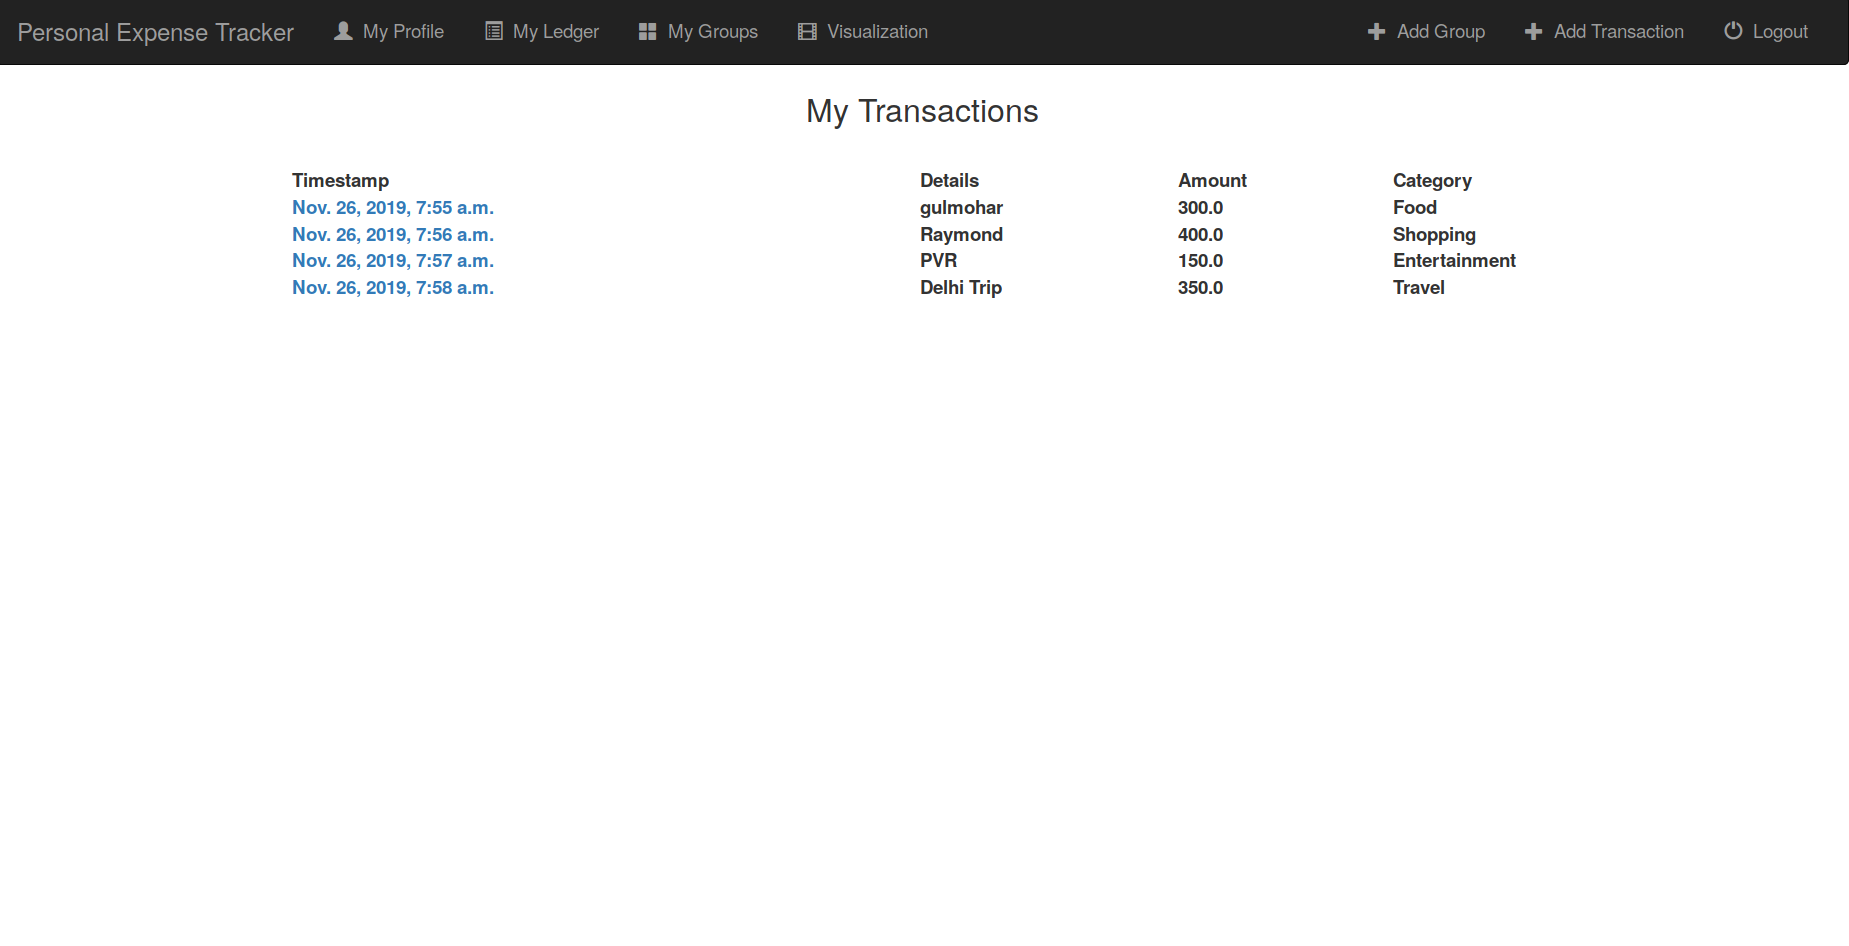
\includegraphics[height=8cm]{ledger.png}
            \caption{Transaction details for a user}
            \label{fig:my_label}
        \end{figure}

    \item \textbf{graphs}:- This module provides better visualization in the form of pie and bubble charts.
    \begin{figure}[tb]
        \begin{subfigure}[t]{1\hsize}
            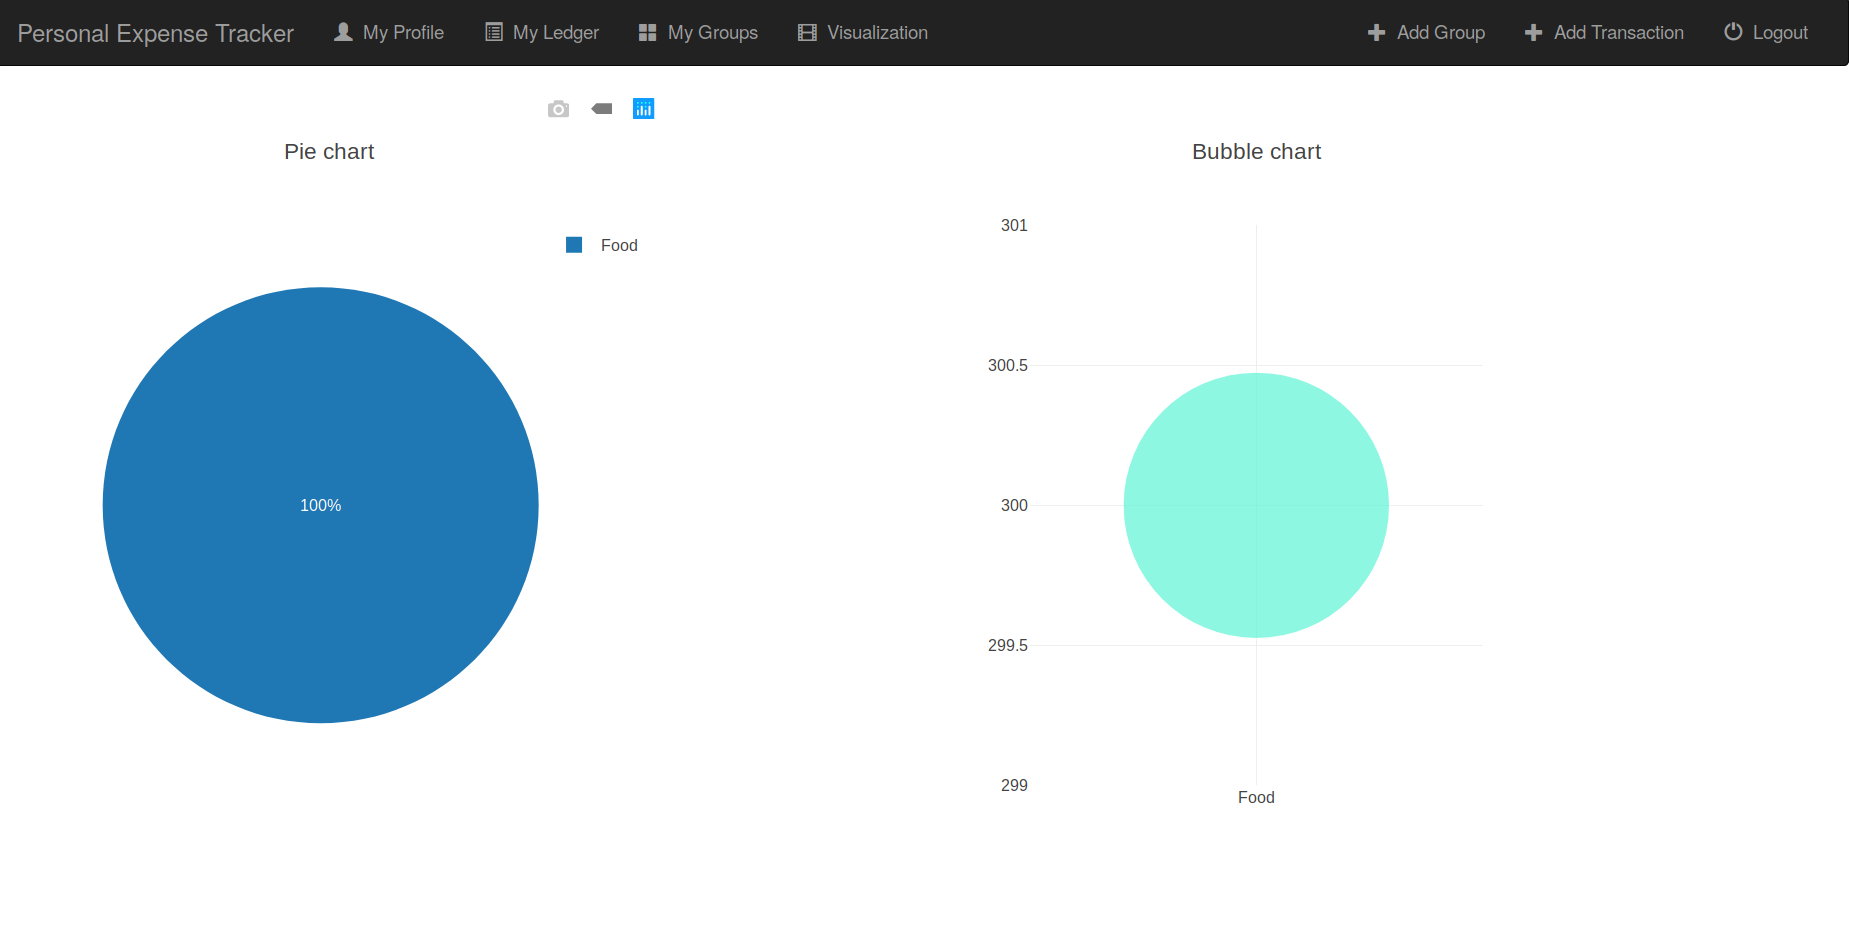
\includegraphics[width=0.9\linewidth]{visualize1.png}
            \caption{Graphs after first transaction}
        \end{subfigure}   
        \begin{subfigure}[t]{1\hsize}
            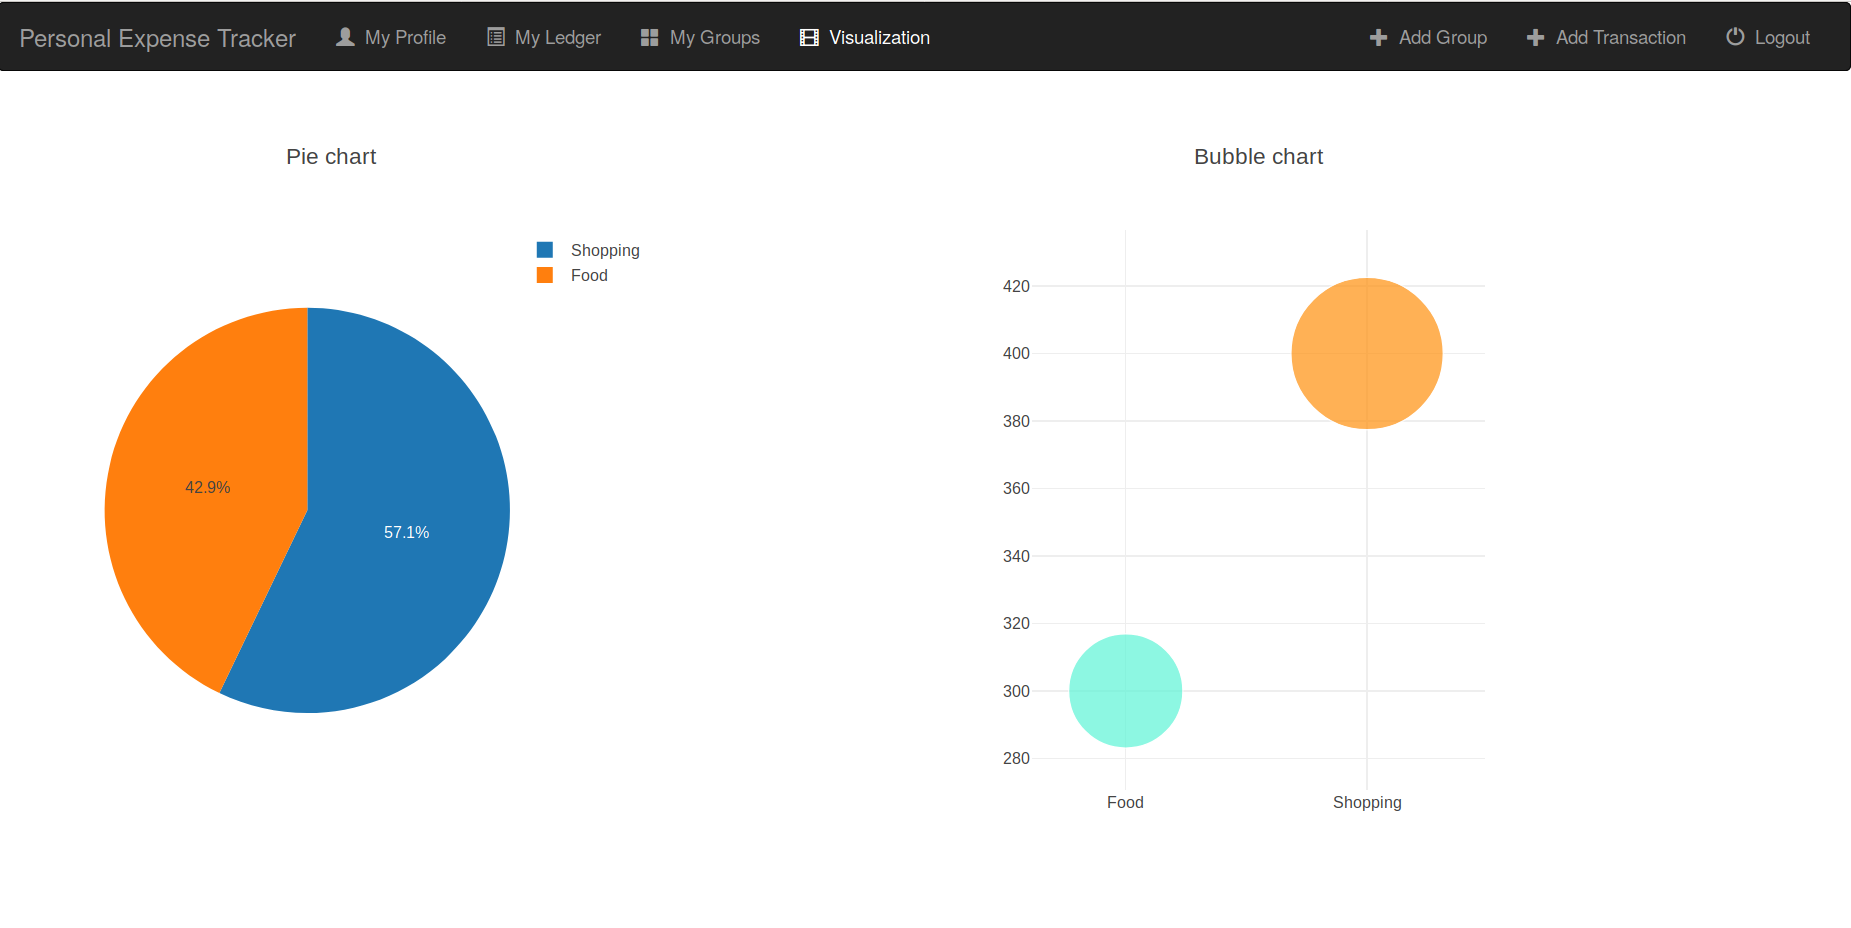
\includegraphics[width=0.9\linewidth]{visualize2.png}
            \caption{Graphs after second transaction}
        \end{subfigure}
            \end{figure}
            \clearpage
            \begin{figure}[tb]\ContinuedFloat
        \begin{subfigure}[t]{1\hsize}
            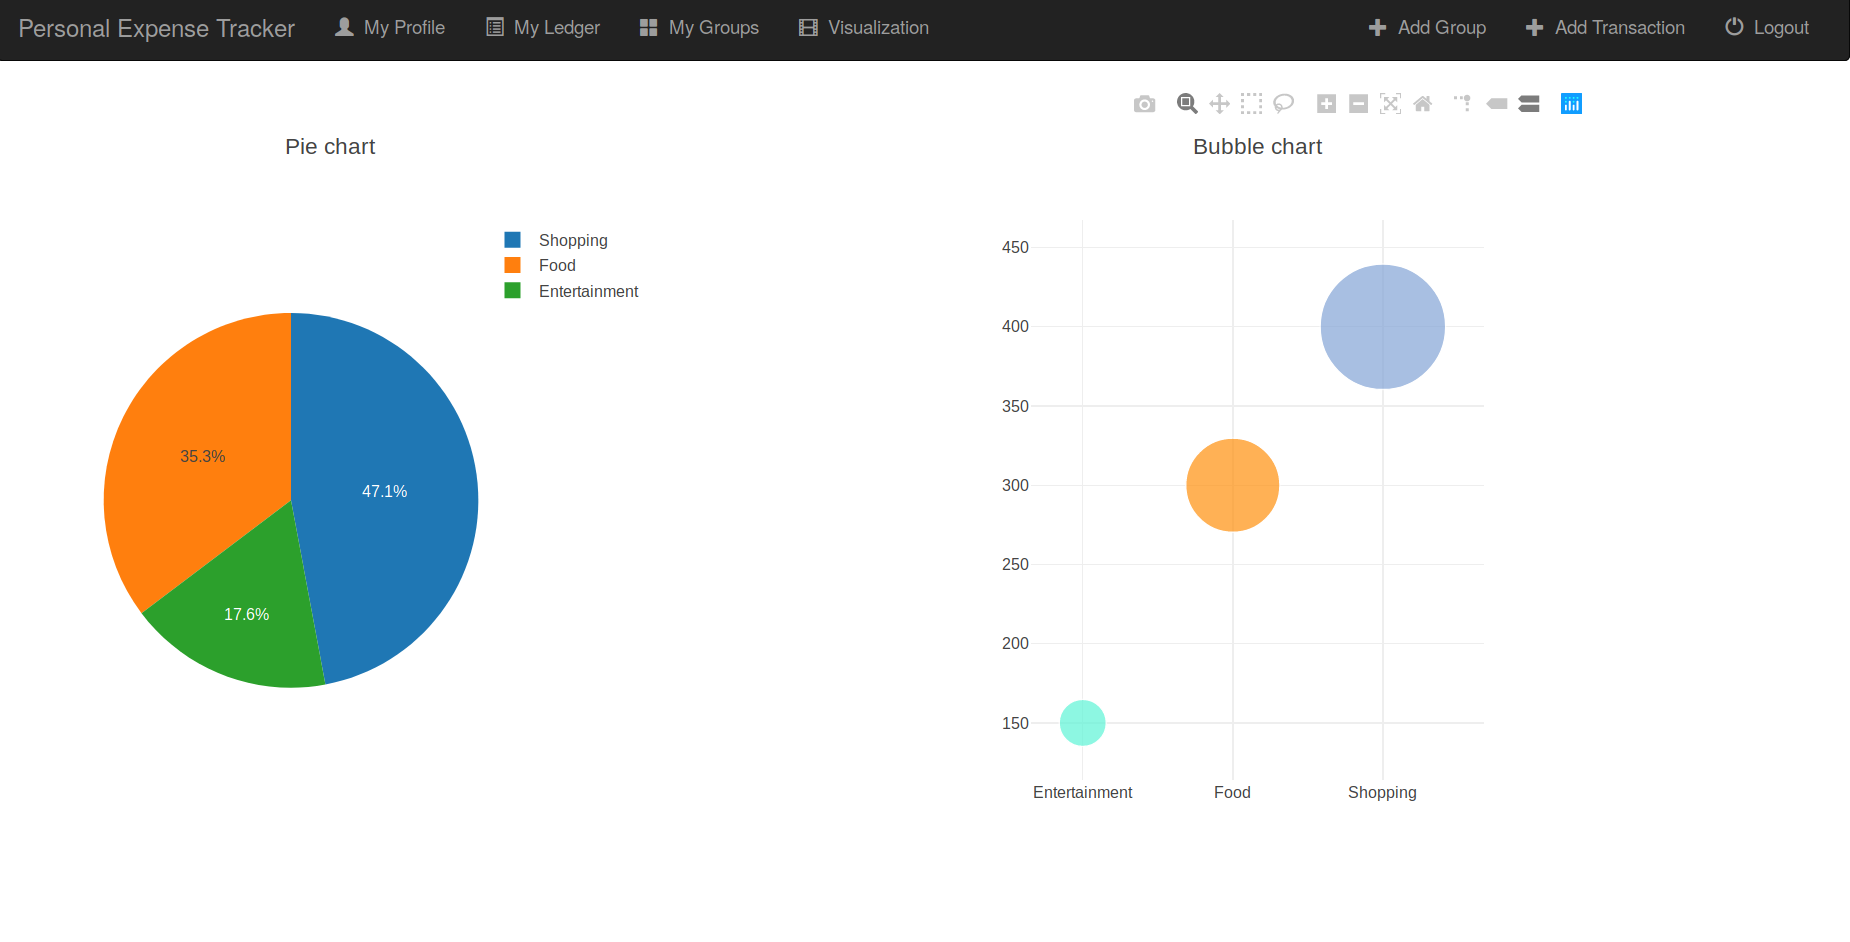
\includegraphics[width=0.9\linewidth]{visualize3.png}
            \caption{Graphs after third transaction}
        \end{subfigure}

    \caption{Visualization of expenses in each domain}
    \end{figure}
    \item \textbf{split}:- This module maintains user groups and their transactions. It also provides algorithm from optimizing group transactions in such a way that there is a minimum-cash flow.
    \begin{figure}[!hb]
        \begin{subfigure}[t]{0.5\hsize}
            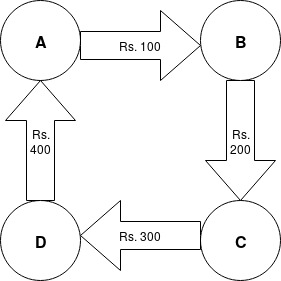
\includegraphics[width=0.9\linewidth]{Cycle.jpg}
            \caption{Cycles in Group}
        \end{subfigure}   
        \begin{subfigure}[t]{0.5\hsize}
            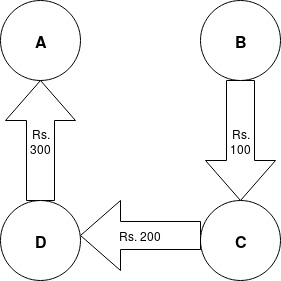
\includegraphics[width=0.9\linewidth]{Cycle_break.jpg}
            \caption{Cycle removed after optimizing the group transactions}
        \end{subfigure}
            \caption{Minimum cash flow}
    \end{figure}

    \item \textbf{OCR}:- Takes image as input, process it and output the bill details.
    \begin{figure}[!ht]
        \centering
        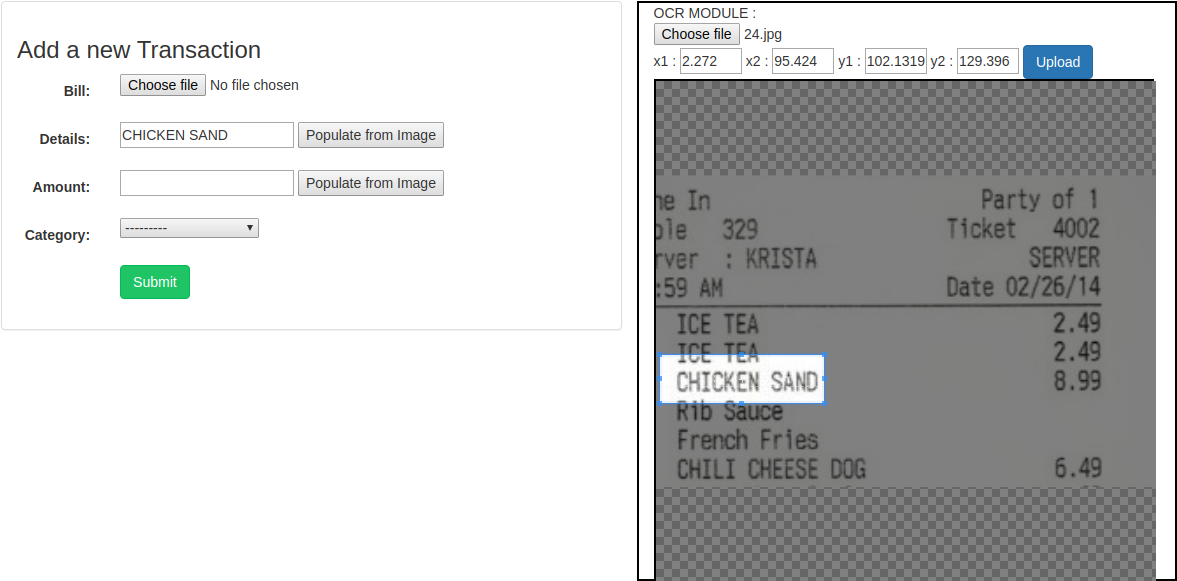
\includegraphics[width=0.9\linewidth]{ocr.png}
        \caption{Text extracted through OCR}
        \label{fig:my_label}
    \end{figure}
\end{enumerate}


\pagebreak

\section{FEATURES}
\begin{itemize}
    \item Interactive Web UI - A rich user interface with buttons to add transactions and view transaction history including bills and spending. It also has features to delete and edit transactions.
    
    \item Split Bills - Group finances are handled using this feature (Who-owes-whom etc). In a group, always the minimum cash flow summary is displayed. There are options to settle the debts within a group.
    
    \item OCR - Ability to upload bill details directly from the bill receipts using OCR. Items and their prices can be uploaded using OCR directly by cropping required area.
    
    \item Analysis - Visualization of spending in various domains like Entertainment, Food, Travel, etc. using a pie chart, bubble chart, etc.
\end{itemize}


\newpage
\section{TECHNOLOGIES USED}
\begin{itemize}
    \item Python3
    \item Django
    \item HTML/CSS/JS
    \item SQLite3
    \item \LaTeX
\end{itemize}

\section{LIBRARIES USED}
\begin{itemize}
    \item Tesseract
    \item PIL
    \item Numpy
    \item Plotly
    \item Cropper.js
\end{itemize}



\pagebreak

\section{APPROACH}
\begin{itemize}
    \item The main challenging part of the project was to come up with an efficient way to detect cycles ( Cycles? Here? Say in a group, A owe amount x to B, B owe amount y to C, C owe amount z to A) among the group participants. It would be very inefficient if we revert the transactions to handle the issue, just imagine how inefficient would it become as the number of participants increases within a  group. 
    \item In order to handle this problem, we fetch out the summary for each individual in the group i.e. how much a person owes or how much others owe to that person. Based on the summary, our algorithm finds out what minimum amount needs to be transferred from one individual to another(minimum cash flow) so as to settle up the finances.
    \item The thing which distinguishes it from the existing products is, apart from tracking finances in groups it even allows users to keep track of their individual expenditures (i.e. a personal ledger) in which a user can see the entire list of the transaction he has done with time and category specified( when and where).
    \item The next thing we wanted to have is the flexibility for the user to directly upload bill receipts rather than explicitly typing each and individual entry they spent on. The OCR feature allows cropping out an important section of the bill and then calls python script(which uses tesseract library) to extract out the details in the text format.
    \item Here comes the fun part, a better visualization! As we know numbers are not always the best way to see what's happening around. We get better insights when we can visualize things. So we have charts to offer like, bubble chart and pie chart to show what percentage of your spending is their on what category.


\end{itemize}


\pagebreak


\section{SYSTEM ARCHITECTURE}

\begin{figure}[!ht]
\centering
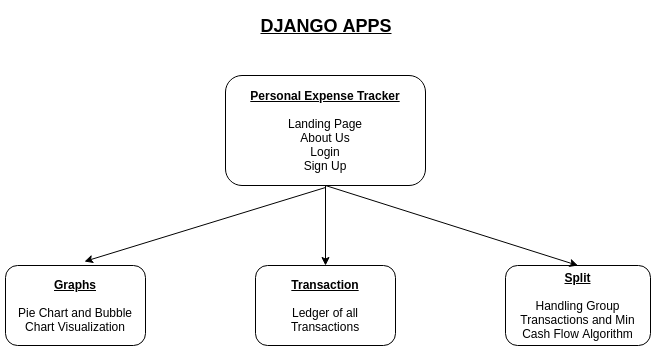
\includegraphics[height=3.5in]{Django_Apps.png} 
\caption{Django App}
\end{figure}
\newline
In Django, it is good practice to break every feature into a new app. So, we have broken the project into 5 apps.
\newline
\begin{itemize}
    \item Personal Expense Tracker - It contains the landing page, all functionality related to login, signup, logout, etc and all base templates which are extended in other modules. It also contains all static files that are used in the project like Images, Javascript and CSS.
    \item Graphs - It contains the graph plotting functionality. Currently we are plotting two types of graphs : (a)Pie Chart (b)Bubble Chart. The data from these graphs is taken from the transactions of the particular user.
    \item Transaction - This module handles everything about the transactions of a user. It stores the bill, category and amount of every transaction added by the user along with the timestamp. 
    \item Split - This module handles the Groups and Settling Debts within a group. 
    \item OCR - This module handles automatic population of transaction fields using bills and Optical Character Recognition. We have used Tesseract and Python Image Library to accomplish this task.
    
\end{itemize}

\vspace{50px}
\begin{figure}[!ht]

\centering
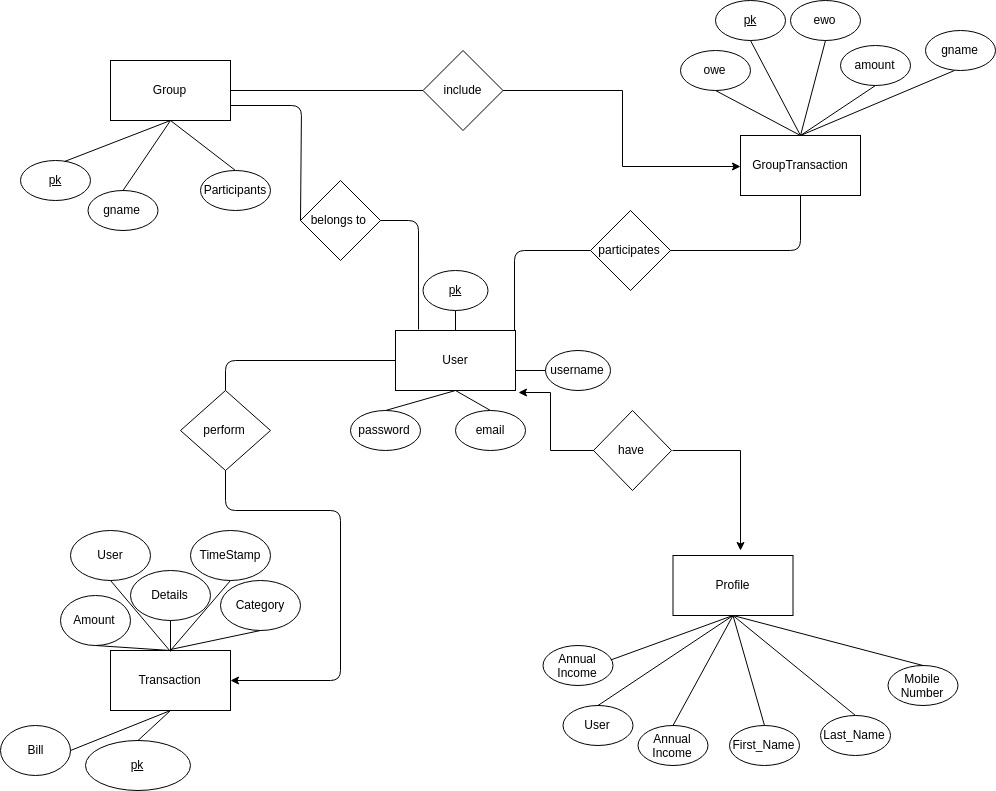
\includegraphics[height=5in]{ERdiagram.jpg}
\caption{ER Diagram}

\end{figure}

\pagebreak

\section{USER DOCUMENTATION}
\begin{itemize}
    \item DJango installation in Linux
    \begin{itemize}
        \item Install a Python Virtual Environment\\
		python3 -m venv $<$environment-name$>$
        \item Activate Virtual Environment\\
		source bin/activate/$<$environment-name$>$
        \item Install Django\\
		pip3 install django
    \end{itemize}
    \item Tesseract installation in Linux \\
    	pip3 install pytesseract
    \item PIL installation in Linux \\
	python3 -m pip install Pillow
	
	\item cd to Sl$\_$proj. You will find a manage.py file over there.
\item run the command 
    python3 manage.py runserver <PORT>
\item go to 127.0.0.1/<PORT> on your browser. You will find yourself on the landing page of the website.
\item Now create a new profile by clicking on Sign Up and entering your details.
\item You can now add Transactions and manage your groups using the button on the navigation bar.
\item You can also view your spending in various domains by looking at the visualization in navbar.
\item You can log out when your work is complete.

\end{itemize}

\pagebreak

\section{FUTURE SCOPE}
There is scope for improvement in the application. The UI can be made more interactive along with aesthetic improvement of the page designs. This is would require work by a Web Designer who has knowledge of the intricacies.

The OCR feature can also be improved to auto populate the fields with items in the bill. It would require significant work in Machine Learning, Natural Language Processing and Image Processing to recognize relevant entities in the bill accurately.

Other than these two things, any new feature can also be added, depending on specific needs of the user.

\section{NOVELTY}
Comparing with the currently available alternatives, our app provides minimum cash flow and better visualization without even charging you a single penny. Group Management and OCR is available in our app which is not available in other apps free of cost.

Our project can be used by students of IIT Bombay for managing their finances for better utilization of pocket money or stipend.

\newpage
\section{CONCLUSION}

We have successfully built a webapp, Personal Expense Tracker which can serve the financial management needs of a person. A rich set of features such as group splitting, graphical visualization and Optical Character Recognition to automatically populate the fields using the receipt along with basic ledger functionality make for a wholesome experience.

The application has been built in a modular manner following software design principles which offer privacy, correctness and extensibility for new features.




\newpage
\bibliographystyle{plain}
\bibliography{biblist}

\end{document}
